\thispagestyle{scrheadings}
\section{Allgemeiner Aufbau von Hexapod-Kinematiken}
\label{basics-aufbau}

\begin{figure}[!htb]
    \centering
    \includegraphics[width=0.7\textwidth]{basics/stab1}
    \caption[Folie]{Folie, Quelle: Eigene Darstellung}
    \label{fig:stab1}
\end{figure}

\begin{figure}[H]
    \centering
    \includegraphics[width=0.7\textwidth]{basics/stab2}
    \caption[Folie]{Folie, Quelle: Eigene Darstellung}
    \label{fig:stab2}
\end{figure}

\begin{figure}[H]
    \centering
    \includegraphics[width=0.7\textwidth]{basics/stab3}
    \caption[Folie]{Folie, Quelle: Eigene Darstellung}
    \label{fig:stab3}
\end{figure}

\begin{figure}[H]
    \centering
    \includegraphics[width=0.7\textwidth]{basics/stab4}
    \caption[Folie]{Folie, Quelle: Eigene Darstellung}
    \label{fig:stab4}
\end{figure}

\begin{figure}[H]
    \centering
    \includegraphics[width=0.7\textwidth]{basics/stab5}
    \caption[Folie]{Folie, Quelle: Eigene Darstellung}
    \label{fig:stab5}
\end{figure}

\thispagestyle{scrheadings}
\section{Mathematische Modellierung}
\label{basics-modelling}

\begin{figure}[H]
    \centering
    \includegraphics[width=0.7\textwidth]{basics/kin1}
    \caption[Folie]{Folie, Quelle: Eigene Darstellung}
    \label{fig:kin1}
\end{figure}

\subsection{Transformationsgleichungen}
\label{basics-transformation}

\begin{figure}[H]
    \centering
    \includegraphics[width=0.7\textwidth]{basics/kin2}
    \caption[Folie]{Folie, Quelle: Eigene Darstellung}
    \label{fig:kin2}
\end{figure}

\begin{figure}[H]
    \centering
    \includegraphics[width=0.7\textwidth]{basics/kin3}
    \caption[Folie]{Folie, Quelle: Eigene Darstellung}
    \label{fig:kin3}
\end{figure}

\begin{figure}[H]
    \centering
    \includegraphics[width=0.7\textwidth]{basics/kin7}
    \caption[Folie]{Folie, Quelle: Eigene Darstellung}
    \label{fig:kin7}
\end{figure}

\subsection{Transformationskette einer allgemeinen Hexapod-Kinematik}
\label{basics-chain_of_transformation}

\begin{figure}[H]
    \centering
    \includegraphics[width=0.7\textwidth]{basics/kin4}
    \caption[Folie]{Folie, Quelle: Eigene Darstellung}
    \label{fig:kin4}
\end{figure}

\begin{figure}[H]
    \centering
    \includegraphics[width=0.7\textwidth]{basics/kin5}
    \caption[Folie]{Folie, Quelle: Eigene Darstellung}
    \label{fig:kin5}
\end{figure}

\begin{figure}[H]
    \centering
    \includegraphics[width=0.7\textwidth]{basics/kin6}
    \caption[Folie]{Folie, Quelle: Eigene Darstellung}
    \label{fig:kin6}
\end{figure}

\subsection{Bestimmung der wirkenden Kräfte}
\label{basics-forces}

\begin{figure}[H]
    \centering
    \includegraphics[width=0.7\textwidth]{basics/force1}
    \caption[Folie]{Folie, Quelle: Eigene Darstellung}
    \label{fig:force1}
\end{figure}

\begin{figure}[H]
    \centering
    \includegraphics[width=0.7\textwidth]{basics/force2}
    \caption[Folie]{Folie, Quelle: Eigene Darstellung}
    \label{fig:force2}
\end{figure}

\begin{figure}[H]
    \centering
    \includegraphics[width=0.7\textwidth]{basics/force3}
    \caption[Folie]{Folie, Quelle: Eigene Darstellung}
    \label{fig:force3}
\end{figure}

\begin{figure}[H]
    \centering
    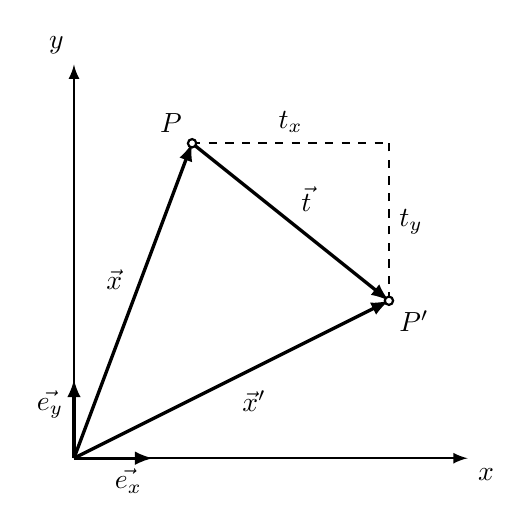
\begin{tikzpicture}[scale = 1]
    \sansmath
    
    \begin{scope}[thick,->,>=latex]
    \draw (0,0) -- (5,0) node[anchor=north west] {$x$};
    \draw (0,0) -- (0,5) node[anchor=south east] {$y$};
    \end{scope}
    
    \begin{scope}[very thick,->,>=latex]
    \draw (0,0) -- (1,0) node[anchor=north east] {$\vec{e_{x}}$};
    \draw (0,0) -- (0,1) node[anchor=north east] {$\vec{e_{y}}$};
    \end{scope}
    
    \coordinate (O) at (0,0);
    \coordinate (P1) at (1.5,4);
    \coordinate (P2) at (4,2);
    
    \begin{scope}[very thick,->,>=latex]
    \draw (O) -- (P1) node [midway, anchor = south east] {$\vec{x}$};
    \draw (O) -- (P2) node [midway, anchor = north west] {$\vec{x}^\prime$};
    \draw (P1) -- (P2) node [midway, anchor = south west] {$\vec{t}$};
    \end{scope}
    
    \begin{scope}[thick, dashed]
    \draw (P1) -- (4,4) node [midway, anchor = south] {$t_{x}$};
    \draw (P2) -- (4,4) node [midway, anchor = west] {$t_{y}$};
    \end{scope}
    
    \begin{scope}[thick,draw=black,fill=white]
    \filldraw (P1) circle (1.5pt) node[anchor=south east] {$P$};
    \filldraw (P2) circle (1.5pt) node[anchor=north west] {$P^\prime$};
    \end{scope}
    
    \end{tikzpicture}
    \caption[Abbildung]{Abbildung, Quelle: Eigene Darstellung}
    \label{fig:force3}
\end{figure}